\documentclass{beamer}
\usepackage[russian]{babel}
\usepackage[utf8]{inputenc}
\usepackage{listings}
\usepackage{minted}


\usetheme[pageofpages=/,% String used between the current page and the
                         % total page count.
          bullet=circle,% Use circles instead of squares for bullets.
          titleline=true,% Show a line below the frame title.
          alternativetitlepage=false,% Use the fancy title page.
          watermark=aupic,% Watermark used in every page.
          watermarkheight=60px,% Height of the watermark.
          watermarkheightmult=4,% The watermark image is 4 times bigger
                                % than watermarkheight.
          ]{Torino}

\author{выполнил Андрей Серебро\\
руководитель Илья Бирюков (JetBrains)}
\title{Стратегии подстановки макросов в C++}
\institute{Санкт-Петербургский Академический Университет}
\date[b]{20 мая 2016}
  
\definecolor{darkgreen}{rgb}{0,0.5,0}
\definecolor{dhscodebg}{rgb}{0.95,0.95,0.95}
\newminted[dhscode]{c++}{tabsize=4, fontsize=\footnotesize, frame=lines, framesep=5\fboxrule,framerule=1pt,
bgcolor=dhscodebg, rulecolor=\color{gray!40}}

\newcommand\hideit[1]{%
  \only<0| handout:1>{\mbox{}}%
  \invisible<0| handout:1>{#1}}

\begin{document}



\defverbatim[colored]\lstI{
\begin{lstlisting}[language=C++,basicstyle=\ttfamily,keywordstyle=\color{blue},commentstyle=\color{darkgreen}]
#define M1 1
#define M2 M1
#define M3 M2
...
int x = M3 + M3; // M3 expands two times
\end{lstlisting}
}

\defverbatim[colored]\lstRepeat{
\begin{lstlisting}[language=C++,basicstyle=\ttfamily,keywordstyle=\color{blue},commentstyle=\color{darkgreen},basicstyle=\small]
#define BOOST_PP_REPEAT_1_0(m, d)
#define BOOST_PP_REPEAT_1_1(m, d) m(2, 0, d)
#define BOOST_PP_REPEAT_1_2(m, d) \ 
           BOOST_PP_REPEAT_1_1(m, d) m(2, 1, d)
...
#define BOOST_PP_REPEAT_1_255(m, d) \
           BOOST_PP_REPEAT_1_254(m, d) m(2, 3, d)
\end{lstlisting}
}

\defverbatim[colored]\lstCat{
\begin{lstlisting}[language=C++,basicstyle=\ttfamily,keywordstyle=\color{blue},commentstyle=\color{darkgreen}]
#define CAT1(X, Y) X ## Y
#define CAT2(X, Y) CAT1(X, Y)
#define MACRO 1
CAT1(MACRO, 0) // MACRO0, not 10 
CAT2(MACRO, 0) // 10
\end{lstlisting}
}


\defverbatim[colored]\argCat{
\begin{lstlisting}[language=C++,basicstyle=\ttfamily,keywordstyle=\color{blue},commentstyle=\color{darkgreen}]
#define ARG 2
#define M(ARG) ARG + A##RG
M(3) // 3 + 2
\end{lstlisting}
}

\defverbatim[colored]\invalidCache{
\begin{lstlisting}[language=C++,basicstyle=\ttfamily,keywordstyle=\color{blue},commentstyle=\color{darkgreen},basicstyle=\fontsize{8}{9}\ttfamily]
// in boost/preprocessor/detail/check.hpp
#define BOOST_PP_CHECK_D(x, type)  \
    BOOST_PP_CHECK_1(BOOST_PP_CAT(BOOST_PP_CHECK_RESULT_, type x))
#define BOOST_PP_CHECK_1(chk) BOOST_PP_CHECK_2(chk)
#define BOOST_PP_CHECK_2(res, _) res

#define BOOST_PP_CHECK_RESULT_1 1, BOOST_PP_NIL
...
int a = BOOST_PP_CHECK_D(1,); // must compile!
\end{lstlisting}
}

\begin{frame}[t,plain]
\titlepage
\end{frame}

\begin{frame}[t, fragile]{Мотивация}
\begin{itemize}
\item При повторной подстановке макроса всё время
делается одна и та же работа
\item Можно ли ускорить препроцессирование, если
сделать её только один раз?
\end{itemize}

\lstI

\end{frame}

\begin{frame}[t, fragile]{Мотивация}
Когда лексинг может быть медленным
\begin{itemize}[<+->]
\item Загрузка в IDE большого проекта
\item Много метапрограммирования (например, Boost.Preprocessor)


\lstRepeat

\end{itemize}
\end{frame}


\begin{frame}[t, fragile]{Подход}
Попробуем кешировать результат раскрытия макроса
\begin{itemize}[<+->]
\item Построение кеша = разбор на лексемы тела макроса с максимальным <<упрощением>> результата
\begin{itemize}
\item Ленивое: пока не случилось первое раскрытие, ничего не делаем
\item Очень просто для объектного макроса
\item Очень просто для функционального макроса, игнорирующего свои аргументы
\item Функциональный макрос использующий аргументы - единственный сложный кейс
\end{itemize}
\item Инвалидация
\end{itemize}

\end{frame}

\begin{frame}[t, fragile]{Построение кеша функционального макроса}
\begin{itemize}
\item При кешировании нельзя раскрывать токены-аргументы
\argCat
Кеш должен содержать ARG + 2\\
Решается булевским флажком "токен - аргумент"
\end{itemize}
\end{frame}

\begin{frame}[t, fragile]{Построение кеша функционального макроса}
\begin{itemize}[<+->]
\item Обычно при подстановке в макрос аргумент полностью раскрывается
\item Кроме случаев, когда аргумент макроса соседится с конкатенирующим токеном \#\# или стрингифицирующим \# слева
\item К чему это приводит в нашем случае?
\end{itemize}

\end{frame}

\begin{frame}[t, fragile]{Построение кеша функционального макроса}

\lstCat
\begin{itemize}[<+->]
\item Кеш для CAT2 очевидно не может быть X \#\# Y

\item Решаем, заведя пару специальных токенов [ и ]. всё что между парой таких токенов, должно быть раскрыто.
\item CAT1 = X \#\# Y\\
\item CAT2 = [X] \#\# [Y]
\end{itemize}
\end{frame}

\begin{frame}[t, fragile]{Инвалидация}
Когда сбрасывать кеш?
\begin{itemize}[<+->]
\item Когда макрос переопределён
\item Когда какой-то макрос, встречавшийся в ходе разбора макроса, переопределён
\item Когда какой-то идентификатор, встречавшийся в ходе разбора макроса, становится определён как макрос
\end{itemize}


\only<4>{На данный момент энергичная инвалидация при переопределениях, ленивая при новом определении}
\end{frame}



\begin{frame}[t, fragile]{Когда кешировать вредно}

\begin{itemize}[<+->]
\item Существуют случаи, когда кеширование приводит к генерации невалидного кода
\item Например, когда так:
\invalidCache
\item Проблема: кеширование BOOST\_PP\_CHECK\_1 $\Rightarrow$ ошибка!
\item Решение: случилась ошибка $\Rightarrow$ запретить кеш
\end{itemize}
\end{frame}

\begin{frame}[t, fragile]{Результаты}
\begin{itemize}[<+->]
\item Взят clang, release 38. К нему применён описанный патч. 
\item На данный момент пожертвовали диагностическими данными о точках раскрытия (SourceLocation) :( 
\item Можно добавить флажок в clang или подумать как спасти диагностику
\item Репозиторий: \url{https://github.com/Aspirisha/clang/tree/macros_patch}
\item Препроцессинг всех хедеров Boost 1.54.0.1:
\begin{center}
\begin{tabular}{|c|c|c|}
\hline
Clang & Clang (без SourceLocation) & Clang hacked \\
\hline
1331 c & 1099 c (на 17\% быстрее) & 782 c (на 41\% быстрее) \\
\hline
\end{tabular}
\end{center}
\end{itemize}

\end{frame}

\begin{frame}[t, fragile]{Статистика}
\begin{itemize}[<+->]
\item Среднее по бустовым хедерам ускорение в 1.4 раза
\item Самый значительный прирост в скорости на boost/mpl/string.hpp - в 4 раза
\item 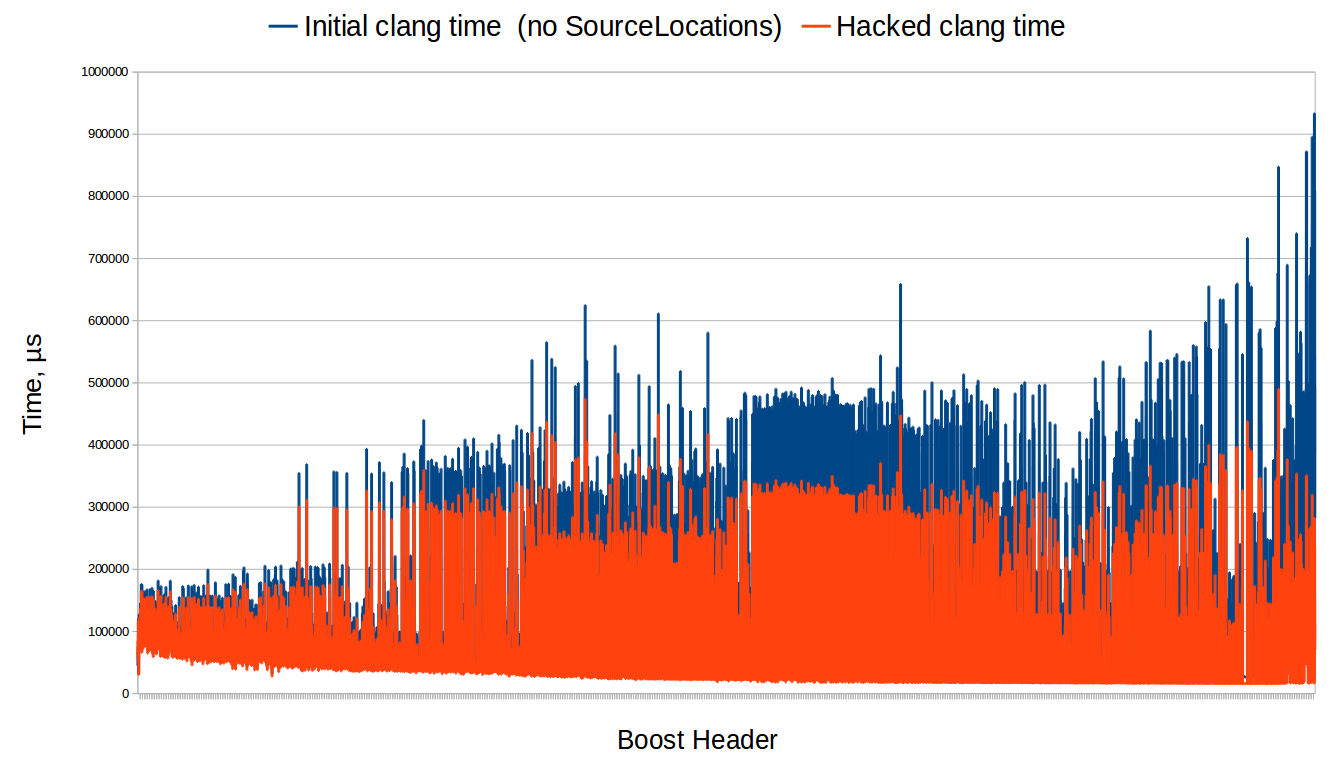
\includegraphics[scale=0.2]{graph1}

\end{itemize} 
\end{frame}





\begin{frame}[t, fragile]{Очень интересно, и что дальше?}
\begin{itemize}[<+->]
\item В марте создан тред на cfe-dev по поводу ускорения препроцессора:
\url {http://clang-developers.42468.n3.nabble.com/Re-llvm-dev-Clang-Preprocessor-Speed-Up-td4050728.html}
\begin{itemize}
\item Ребята отнеслись скептически
\item На этой неделе туда отправлен патч
\end{itemize} 
\item Проводить дезинсекцию (увы, Boost 1.61.0 содержит примеры, на которых валится, например boost/log/support/spirit\_qi.hpp)
\item Цель-максимум - доотладить и PR
\end{itemize} 

\end{frame}

\begin{frame}[fragile]{Спасибо за внимание}

\begin{center}
\Huge Вопросы, предложения, критика?
\end{center}
\end{frame}

\end{document}

